\documentclass[journal]{IEEEtran}
\usepackage{listings}
\ifCLASSINFOpdf
  \usepackage[pdftex]{graphicx}
  \usepackage{amsfonts}
  % declare the path(s) where your graphic files are
  \graphicspath{{../pdf/}{../jpeg/}}
  % and their extensions so you won't have to specify these with
  % every instance of \includegraphics
  \DeclareGraphicsExtensions{.pdf,.jpeg,.png}
\else
  % or other class option (dvipsone, dvipdf, if not using dvips). graphicx
  % will default to the driver specified in the system graphics.cfg if no
  % driver is specified.
  \usepackage[dvips]{graphicx}
  % declare the path(s) where your graphic files are
  \graphicspath{{../eps/}}
  % and their extensions so you won't have to specify these with
  % every instance of \includegraphics
  \DeclareGraphicsExtensions{.eps}
\fi
\usepackage{graphics}
\usepackage{float}
\usepackage{caption}
\hyphenation{op-tical net-works semi-conduc-tor}


\begin{document}

\title{Analisando o Desempenho do Sample Sort Paralelo}


\author{Beatriz de Jesus Costa,
        ra104361@uem.br
        e~Bruna Stefany Batista Marques, ra103404@uem.br
}


% The paper headers



\maketitle


\begin{abstract}
For a long time, the search for improving the efficiency of programs and making them execute faster has taken place. This has continued to the present day. This improvement in efficiency has been sought in the most diverse areas and applications. Parallel programming is applied to increase performance, decrease clock execution time, decrease performance per watt and save energy and resources. In this work, a sequential and a parallel version of the Sample Sort algorithm will be implemented, the results will be presented and discussed in relation to the performance of the versions.
\end{abstract}

\def\abstractname{Resumo}
\begin{abstract}
Desde muito tempo, a procura por melhorar a eficiência de programas e tornar sua execução mais rápida acontece, isto estende-se até os dias atuais. Essa melhoria na eficiência vem sendo procurada nas mais diversas áreas e aplicações. A programação paralela é aplicada visando aumentar o desempenho, diminuir o tempo de execução do clock, diminuir o desempenho por watt e economizar energia e recursos. Neste trabalho serão implementadas uma versão sequencial e uma paralela do algoritmo Sample Sort, serão apresentados e discutidos os resultados em relação ao desempenho das versões.
\end{abstract}


\begin{IEEEkeywords}
  Sample Sort, paralelisno, ordenação, programação paralela, desempenho.
\end{IEEEkeywords}


\IEEEpeerreviewmaketitle



\section{Introdução}

\IEEEPARstart{A}busca por melhoria na eficiência dos programas é um problema antigo que se estende até os dias atuais. Cada vez faz-se mais necessário que as aplicações melhorem seus desempenhos para as mais diversas aplicações. Uma das alternativas para conseguir melhorar a eficiência dos programas é a utilização de programação paralela. Um programa paralelo é dividido em vários núcleos em um processador ou conjunto de processadores. Cada subprocesso pode ter seu próprio conjunto de memória, no entanto, também é possível que compartilhe memória com outros processos. 

A necessidade por computação de alto desempenho vem crescendo e os desenvolvedores de hardware estão procurando alternativas como unidades de processamento gráfico (GPUs) e unidades de processamento tensor (TPUs), que dependem da computação paralela para fazer mais coisas ao mesmo tempo. Uma grande parcela dos aumentos de velocidade para computadores de consumo estão relacionadas a melhorias de coordenação de vários núcleos em uma CPU. Apesar disso, adicionar mais núcleos não é o bastante para aumentar a velocidade. Os programadores precisam aprender a escrever programas que aproveitem os recursos dos processadores paralelos.

O objetivo da computação paralela tem sido tradicionalmente fornecer desempenho em termos de potência do processador ou memória que um único processador não pode fornecer; portanto, o objetivo é usar vários processadores para resolver um único problema \cite{lin}.

Segundo os autores Kumar e Gupta (1994), ao resolver um problema em paralelo, é razoável esperar uma redução no tempo de execução que seja comensurável com a quantidade de recursos de processamento empregados para resolver o problema. A escalabilidade de um algoritmo paralelo em um a arquitetura paralela é uma medida de sua capacidade de utilizar efetivamente um número crescente de processadores \cite{Kumar}. 



O objetivo deste trabalho é implementar o algoritmo Sample Sort em uma versão sequencial e em uma versão paralela, realizar experimentos com diferentes entrada de dados e diferentes números de threads  e  analisar o desempenho dos algoritmos para essas entradas. Os algoritmos serão analisados por meio de algumas medidas como speedup e eficiência. 


Analisar a escalabilidade de uma combinação de algoritmo paralelo é muito importante e pode ser usada para diferentes finalidades, como selecionar a melhor combinação de algoritmo e arquitetura para um problema; prever o desempenho de um algoritmo paralelo e uma arquitetura paralela para um grande número de processadores de desempenho conhecido em menos processadores; em um problema de tamanho fixo, pode ser usado para determinar o número ideal de processadores a serem usados; entre outros \cite{Kumar}.

 
\hfill Setembro 30, 2020



\section{Problema}
\label{problema}
Sample Sort é um algoritmo de classificação de divisão e conquista muito utilizado em sistemas de processamento paralelo. Os algoritmos de classificação de divisão e conquista, geralmente particionam a matriz ou vetor em subintervalos que são classificados individualmente e, posteriormente, concatenados. 

Grande parte das abordagens tratam o Sample Sort como uma generalização do algoritmo de ordenação Quicksort. O Sample Sort pega uma amostra maior de sua entrada e divide seus dados em intervalos de acordo. Como o Quicksort, ele classifica recursivamente os intervalos. 

O Sample Sort é mais eficiente em cache do que a classificação rápida porque move os elementos apenas $log(k)$ $n$ vezes, em vez de log n vezes. O parâmetro k depende de várias propriedades da máquina \cite{sanders}.

Uma estratégia muito utilizada no Sample Sort é definir \textit{p} igual ao número de processadores disponíveis. Os dados são então distribuídos entre os processadores, que realizam a classificação dos subvetores usando algum outro algoritmo de classificação sequencial.

Sample Sort é considerado um dos algoritmos baseados em comparação mais eficientes para arquiteturas de memória distribuída \cite{Leischner}. 

Existem três etapas básicas no Sample Sort: encontrar os divisores, que serão os valores que dividem os dados em subvetores; usar os divisores classificados para definir subvetores nos processadores diferentes; colocar os dados nos vetores apropriados; classificar cada um dos subvetores \cite{berlim}.

Os algoritmos implementados nesse trabalho foram inspirados no material do autor BEKTAŞ \cite{slides}.

Na figura \ref{fig:sequencial}, é possível observar um exemplo da execução do Sample Sort sequencial.


\begin{figure*}[!htbp]
    \centering
    \caption{Exemplo de execução do Sample Sort sequencial}
    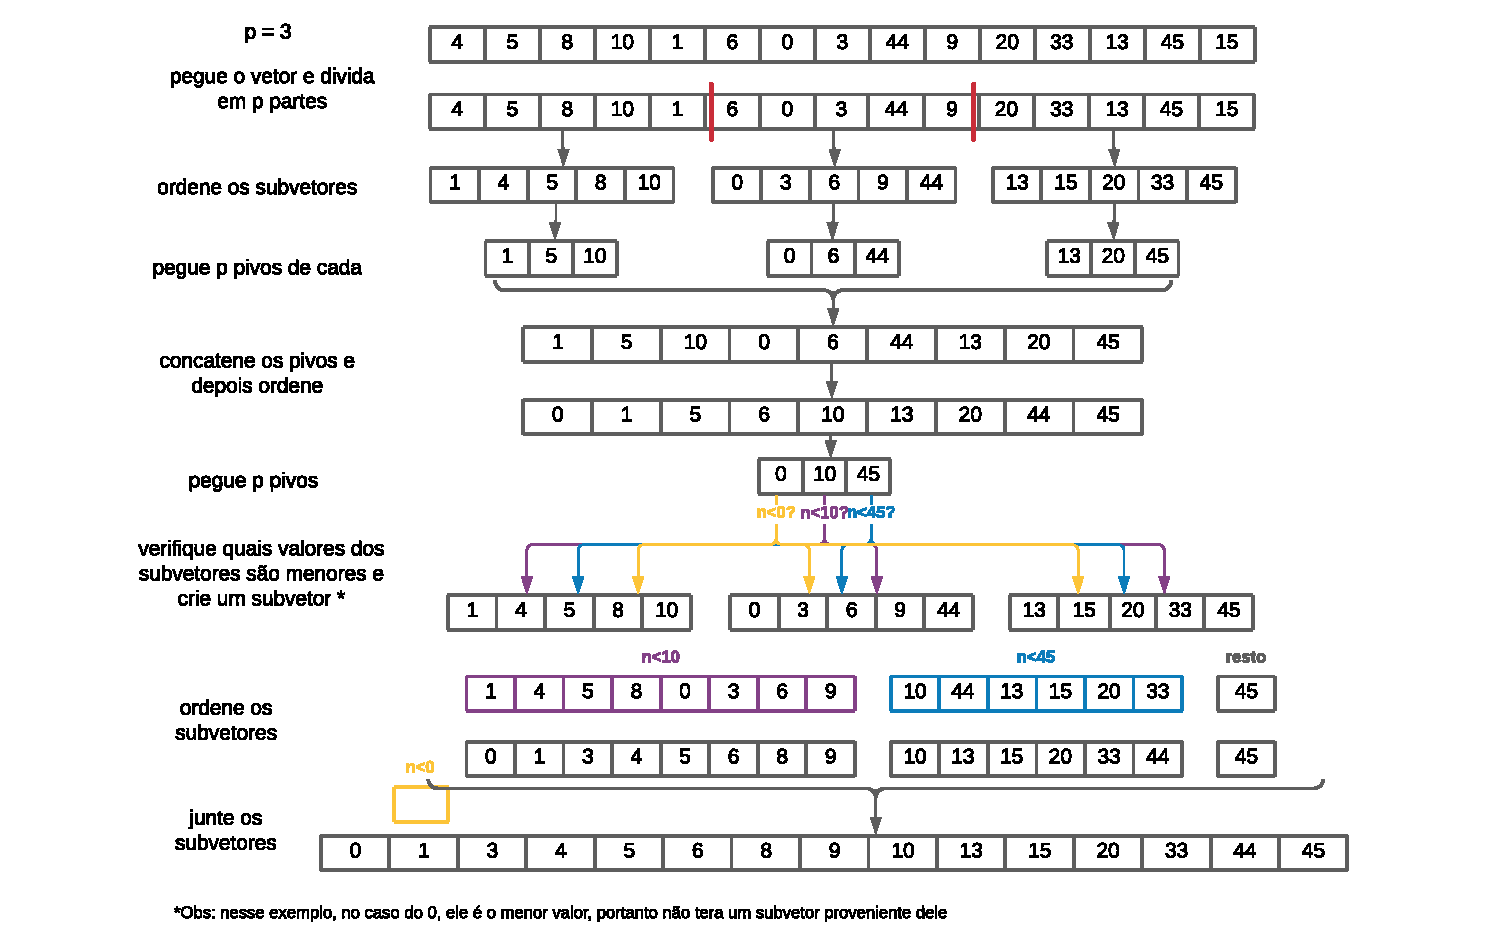
\includegraphics[width=6in]{imagens/samplesortsequencial.pdf}
     \caption*{Fonte: Autoras, 2020}
    \label{fig:sequencial}
\end{figure*}




A ideia por traz do algoritmo é dividir o vetor de entrada de tamanho \textit{n} em {p} subvetores, em que \textit{p} é equivalente ao numero de processadores. Após definir \textit{p} pivôs de cada subvetor para criar um vetor de pivôs. Estes pivôs devem estar uniformemente espaçados para uma melhor performance na ordenação futura. Após essa etapa, são selecionados \textit{p} pivôs uniformemente espaçados deste vetor de pivôs, os pivôs escolhidos são comparados com os subvetores e separados em novos vetores, correspondentes aos números menores do que cada pivô. Após isso esses novos vetores são ordenados e concatenados. Em nossa implementação o número de processadores(p) foi chamado de threads(t) apenas por conveniência. Na seção \ref{formulacao_seq} é possível encontrar um pseudocódigo descrevendo o funcionamento do algoritmo.

\subsection{Formulação}
\label{formulacao_seq}
\begin{table}[H]
    \centering
    \begin{tabular}{|c|}\hline
     \begin{lstlisting} 
    1. Receba um vetor de entrada de tamanho T
       e divida em P partes;
    2. Ordene os subvetores gerados;
    3. Pegue P pivos para cada subvetor;
    4. Concatene e ordene os pivos de todos
       subvetores, gerando um vetor de pivos;
    5. Pegue P pivos do vetor de pivos;
    6. Compare esses P valores com os subvetores
       e separe em novos subvetores os valores que 
       forem menores do que ele;
    7. Pegue os numeros que sobraram e coloque em 
       outro subvetor;
    8. Ordene os subvetores;
    9. Concatene tudo.
\end{lstlisting} \\
         \hline
    \end{tabular}
    \label{tab:pseudo_seq}
\end{table}

\section{Uma solução paralela}

O algoritmo do Sample Sort em sua versão paralela não difere muito da versão sequencial, a principal diferença é que serão utilizadas threads para dividir o trabalho. A ideia geral por trás do Sample Sort é quebrar o trabalho entre vários processadores e cada processador classificar sua parte dos dados \cite{berlim}. 

A paralelização do Sample Sort é implementada dividindo a classificação para cada processador ou thread, onde o número de subvetores é igual ao número de processadores. O Sample Sort é eficiente em sistemas paralelos porque cada processador recebe aproximadamente o mesmo tamanho de subvetor. Como os subvetores são classificados simultaneamente, os processadores concluirão a classificação aproximadamente ao mesmo tempo. Entenda por subvetor como os vetores resultantes da divisão do vetor de entrada. 

Sample Sort é uma generalização do Quicksort que divide a entrada em muitas partes, é conhecida como a melhor comparação prática baseada algoritmo de classificação para computadores paralelos com memória distribuída \cite{sanders}.




A ideia por traz do algoritmo em sua versão paralela, apresentada na figura \ref{fig:paralelo} é basicamente a mesma da aplicada na seção \ref{problema}, a diferença é que os processos serão divididos pelas threads. Basicamente o número de threads será definido pelo número de processadores passados ao programa e cada thread ficará responsável por um subvetor. Após isso, vem a etapa de definir os pivôs de cada subvetor para criar um vetor de pivôs. Na etapa de comparação, os pivôs são comparados com os subvetores e separados em novos vetores, correspondentes aos números menores do que cada pivô. Após isso esses novos vetores são ordenados e concatenados. Cada thread ficará responsável por fazer essas etapas para cada subvetor, com exceção das  etapas de concatenação dos vetores de pivôs e concatenação dos vetores finais, que são feitos por apenas uma das threads.

\begin{figure*}[!htbp]
    \centering
    \caption{Exemplo de execução do Sample Sort paralelo}
    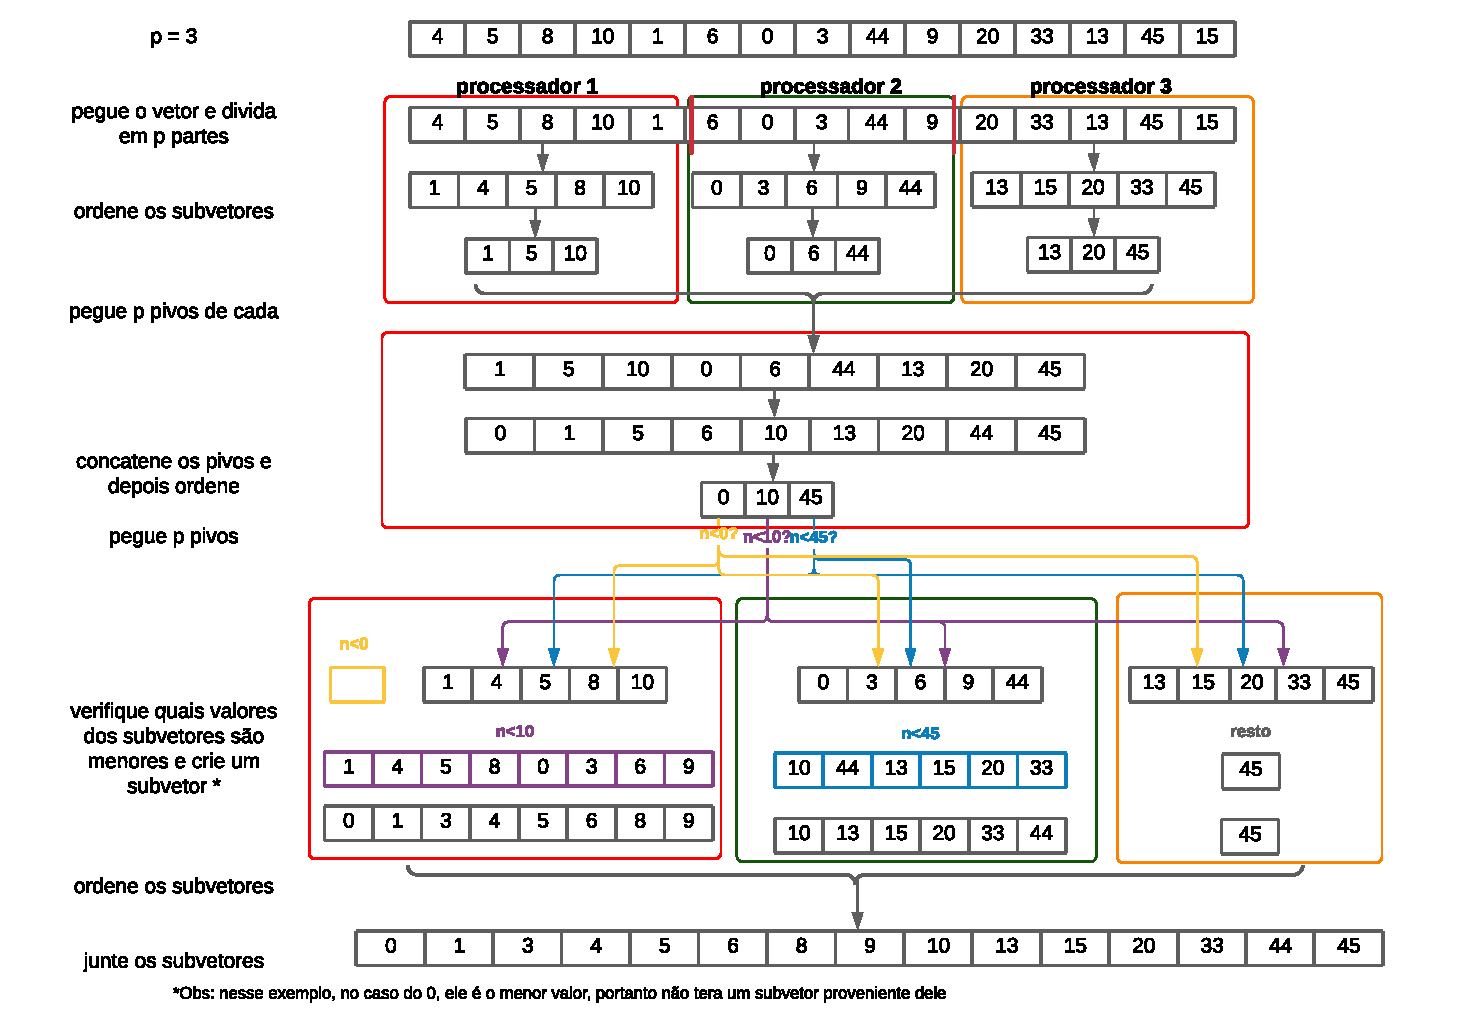
\includegraphics[width=6in]{imagens/samplesortparalelo.pdf}
     \caption*{Fonte: Autoras, 2020}
    \label{fig:paralelo}
\end{figure*}

Vale salientar que foram usadas barreiras entre a etapa de separação dos subvetores, a criação do vetor de pivôs e na etapa de comparação. As barreiras são utilizadas porque na etapa posterior é preciso que os processos de todas as threads tenham sido finalizados. Um exemplo dessa necessidade é na etapa em que os pivôs de cada subvetor são concatenados, se todas as threads não terminarem de ordenar seus subvetores e gerar seus vetores de pivôs, não será possível concatenar os pivôs de todos os subvetores. Para as outras etapas, a necessidade da barreira é basicamente pelo mesmo motivo, ou seja, porque os dados de uma determinada etapa necessitam dos dados da etapa anterior.

 Na figura \ref{fig:paralelo} é possível observar um exemplo de execução do Sample Sort paralelo. Para melhor entendimento, na seção \ref{form_par} é apresentada uma formulação matemática do algoritmo em sua versão paralela. Ao observar a figura pode-se notar como as threads irão funcionar e ter uma ideia da necessidade da utilização de barreiras.




\subsection{formulação}\label{form_par}
\begin{table}[!htbp]
    \centering
    \begin{tabular}{|c|}\hline
         \begin{lstlisting} 
    1. Receba um vetor de entrada de tamanho N
       e divida em P partes, sendo P o numero
       de threads
    2. Ordene os subvetores gerados, cada thread 
       sera responsavel por um subvetor
    3. Pegue P pivos de cada subvetor, cada 
       thread pegara P pivos de seu subvetor
    4. Concatene e ordene os pivos de todos
       subvetores, gerando um vetor de pivos
    5. Pegue P pivos do vetor de pivos
    6. Compare esses P valores com os subvetores
       e separe em novos subvetores os que forem 
       menores do que ele. Cada thread ficara
       responsavel por um subvetor para comparar 
       os pivos
    7. Pegue os numeros que sobraram e coloque em 
       outro subvetor
    8. Ordene os subvetores. Cada thread ficara
       responsavel por um
    9. Concatene tudo.
\end{lstlisting} \\
         \hline
    \end{tabular}
    \label{tab:pseudo_par}
\end{table}
\section{metodologia}
Ambos os algoritmos foram construídos utilizando a linguagem de programação \textit{C}. Para realizar as ordenações durante as etapas do algoritmo, foi utilizado a função \textit{qsort}, das bibliotecas padrões da linguagem. A chamada dessa função aplica o algoritmo de ordenação \textit{Quick Sort} no vetor passado a ela. Para a implementação do algoritmo paralelo foi utilizada a biblioteca \textit{pthread}. Também foi utilizada as funções de barreiras, disponibilizadas pela \textit{pthread}.

Para realizar a avaliação dos algoritmos sequencial e paralelo, foram realizados testes e coletadas medições de desempenho utilizando a ferramenta perf. O algoritmo sequencial foi compilado com o gcc, utilizando as opções de otimização ``-O0'' e ``-O3'', a opção O0 reduz o tempo de compilação e faz com que a depuração produza os resultados esperados, a O3 é o maior nível de otimização, ele tenta reduzir o tamanho do código e o tempo de execução, aumentando o tempo de compilação e o desempenho do código gerado. Vale destacar que otimizar a compilação leva um pouco mais de tempo e muito mais memória para uma função grande. Também foi necessário utilizar a opção "-lm" para realizar a linkagem da biblioteca de matemática, que foi utilizada no código.

As opções do perf que foram selecionadas para coletar as medições foram cache-misses, cycles, instructions, branches, mem-loads, branch-misses, mem-stores, power(energy-pkg); também foi utilizada a opção "-r 10", que executa o código dez vezes e calcula a média das medições das execuções, o que garante maior confiabilidade aos resultados, pois, em alguns algoritmos, a discrepância no desempenho em cada execução pode ser significaiva.
\subsection{Especificações Técnicas}
Os testes foram executados em um notebook Lenovo Ideapad 330. Este computador possui um processador Intel i5-8250U, o que siginifica que o processador é da oitava geração da Intel. O processador possui 8 CPUs, sendo 4 núcleos físicos e 4 virtuais, e frequência de 1,60GHz. Ele conta com 12 GB de memória RAM, 1 T de HD e 120 GB de SSD. Possui também uma GPU Integrada Intel UHD Graphics 620. 
O sistema operacional do computador é o Ubuntu 20.04.1 LTS, com versão GNOME 3.36.3. A versão do gcc instalada foi a 9.3.0. Os códigos foram executados utilizando o terminal padrão do sistema. Vale destacar uma alteração feita para otimização de memória do computador, que foi a mudança da configuração de memória SWAP de 60 para 10, isso significa que anteriormente, quando a memória RAM chegava em 40\% de sua capacidade, alguns pacotes de dados começavam a ser armazenados na memória SWAP, com a alteração essa taxa foi para 90\% da memória RAM, assim o sistema só utiliza o SWAP quando realmente precisa. Essa alteração otimiza o desempenho pois a memória SWAP é mais lenta que a memória RAM, já que é uma quantidade de memória física que é alocada para uso pelo sistema operacional.


\section{Análise e discussão}

\subsection{Speedup}\label{speedup}
Speedup é uma medida de desempenho de dois sistemas processando o mesmo problema. É definido como a proporção do tempo de execução do melhor algoritmo sequencial para resolver um problema pelo tempo gasto pelo algoritmo paralelo para resolver o mesmo problema em um determinado número de processadores, dado pela fórmula $TS/TP$, em que $TS$ diz respeito ao tempo sequencial e $TP$ ao tempo paralelo. É uma das melhores medidas para verificar se o algoritmo paralelo supera o sequencial.

Para os experimentos executados, utilizou-se os otimizadores O0 e O3, para 2,4,8,12 e 16 threads. Nas figuras \ref{fig:speedupO0} e \ref{fig:speedupO3} é possível observar os speedups resultantes das execuções com os otimizadores. Ao analisa-las, foi possível observar que os desempenhos em ambas as otimizações foram muito similares, sendo que na otimização O0, o speedup das primeiras threads foi melhor do que o das últimas. No entanto, os resultados das ultimas threads de O3 foram melhores que os de O0, mas mesmo com essas difreneças, as diferenças entre ambos ainda foi muito pequena. Desta forma, como os resultados foram muito similares, falaremos deles de forma geral.

\begin{figure}[H]
    \centering
    \caption{Speedup O0}
    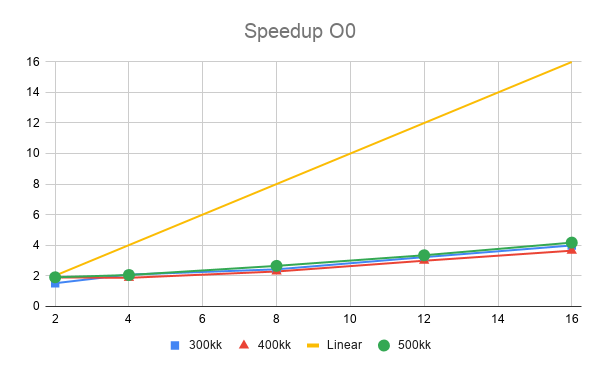
\includegraphics[width=3.7in]{imagens/SpeedupO0.png}
    \caption*{Fonte: Autoras, 2020}
    \label{fig:speedupO0}
\end{figure}

\begin{figure}[H]
    \centering
    \caption{Speedup O3}
    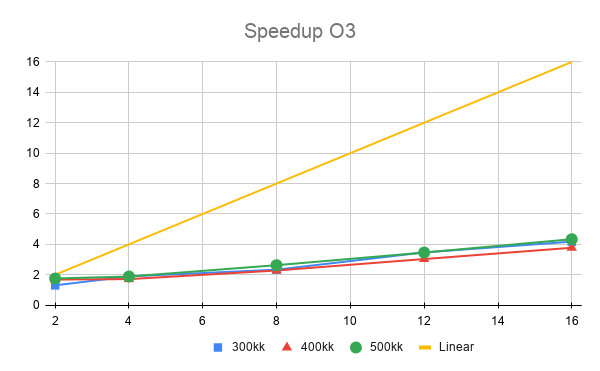
\includegraphics[width=3.7in]{imagens/SpeedupO3.png}
    \caption*{Fonte: Autoras, 2020}
    \label{fig:speedupO3}
\end{figure}

 
Devemos levar em conta que o speedup linear geralmente não é alcançável por causa da contenção por recursos compartilhados, o tempo necessário para se comunicar entre processadores e entre processos, e a incapacidade de estruturar o software para que um um número arbitrário de processadores possa ser mantido utilmente ocupado \cite{Eager}.

Em relação ao speedup, podemos observar que para a thread 2, seu resultado foi muito bom e para 4 foi mediano, no entanto, o resultado das próximas ficam muito distantes do ideal, isso se deve a vários fatores. 

 Tomando como base a explicação dada por Derek et all, uma das justificativas para o speedup ter resultado diferente do ideal é a utilização de barreiras, pois ao utilizá-las forçamos as threadas a esperarem em determinado ponto, o que pode prejudicar o desempenho e tempo de execução. No caso do problema abordado neste trabalho, as barreiras são utilizadas em vários pontos, pois em várias fases do problema é necessário esperar que uma etapa termine para utilizar suas informações na próxima. No entanto, vale salientar que os resultados obtidos não se devem somente as barreiras, elas podem ter sido um dos contribuintes, mas não o único responsável pelos resultados não serem os ideais. Utilizou-se também em um trecho do código os operadores lock e unlock, da biblioteca pthread, na etapa de escrita do vetor ordenado, pois da forma que o problema foi modelado neste trabalho, para que o vetor ordenado retornasse uma saída correta, foi preciso utilizar esse recurso para que as threads escrevessem na ordem correta no vetor final.
 
 Outro fator que pode ter contribuído para os resultados foi a forma que o problema foi modelado, apesar se seguir a ideia principal do algoritmo, pode ter sido implementado de uma forma que menos eficiente. Um dos contribuintes pode ter sido a representação dos subvetores, em que foi utilizada uma matriz para dividir o vetor, no qual cada linha dessa matriz correspondia a um subvetor, a utilização da matriz pode não ter sido a escolha ideal pois para entradas muito grandes a matriz ficará muito grande, sendo custosa para se percorrer e realizar operações com ela. Outro fator que pode ter contribuído é a utilização de somente um vetor para guardar as comparações dos pivôs na etapa de ordenação, em que nestes eram utilizados locks e unloks para controlar a escrita de dados, para que os dados não fossem escritos novamente nas mesmas posições do vetor final. Optamos por utilizar essas estruturas por não ter um controle do tamanho dos subvetores gerados a partir da comparação dos pivôs, no entanto, talvez poderia ser possível a implementação de uma abordagem sem lock e unlock na qual não conseguimos implementar. 
 
 Ainda, segundo a Lei de Amdahl, o speedup de um programa paralelo é limitado pela fração sequencial existente neste programa, ou seja, como usamos barreiras e locks que tornam uma parte do programa sequencial, a Lei de Amdahl afirma que o speedup máximo que a versão paralela atingirá será subtraído pela quantidade de código sequencial existente na versão paralela.
 
 
 Especificidades de implementação como as citadas acima e algumas outras podem ter contribuído para o resultado de speedup mostrado.
 

\subsection{Eficiência}
A eficiência é definida como a utilização média para um número de processadores alocados. Geralmente, a relação entre eficiência e speedup é definida como: $E(n) = S(n)/n$, em que S(n) diz respeito ao speedup e n o número de processadores.

Ao observar os gráficos, nas figuras \ref{fig:eficienciaO0} e \ref{fig:eficienciaO3} podemos observar que os otimizadores não se diferiram muito, da mesmo forma que no speedup. Desta forma, para a eficiência, também iremos analisar os resultados de forma geral. 

A medida que mais processadores são dedicados à execução de um sistema de software, a quantidade total de tempo ocioso do processador pode aumentar, devido a fatores como contenção, comunicação cátion e estrutura de software, e isso pode interferir na eficiência e no speedup de alguns programas.

Em ambos os gráficos \ref{fig:eficienciaO0} e \ref{fig:eficienciaO3}, foi possível observar que a eficiência para a thread 2 foi muito melhor que as outras, o que já era esperado pois na seção \ref{speedup}, foi possível ver que os resultados para a thread 2 foram os que mais chegaram próximos do ideal.



\begin{figure}[H]
    \centering
    \caption{Eficiência utilizando O0}
    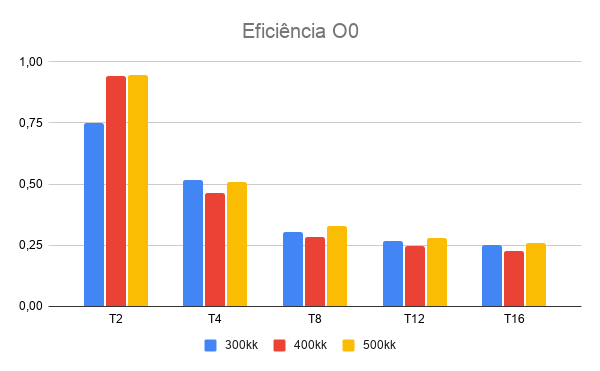
\includegraphics[width=3.7in]{imagens/EficienciaO0.png}
    \caption*{Fonte: Autoras, 2020}
    \label{fig:eficienciaO0}
\end{figure}

\begin{figure}[H]
    \centering
    \caption{Eficiência utilizando O3}
    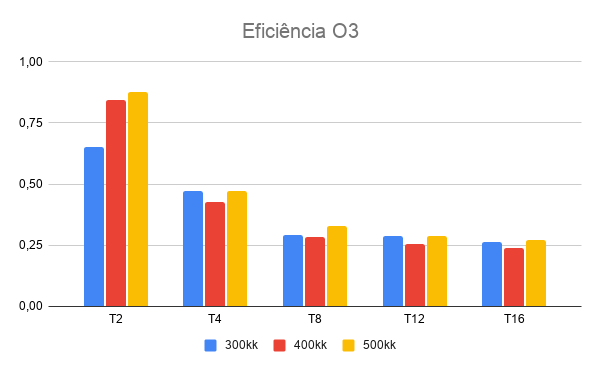
\includegraphics[width=3.7in]{imagens/EficienciaO3.png}
    \caption*{Fonte: Autoras, 2020}
    \label{fig:eficienciaO3}
\end{figure}

Se a eficiência permanecer em 1 conforme os processadores são adicionados, temos aceleração linear \cite{Eager}. Com base nessa definição, podemos observar em nossos gráficos \ref{fig:eficienciaO0} e \ref{fig:eficienciaO3} que a eficiência não permaneceu em 1, o único caso em que ela se aproximou de 1 foi na thread 2, justamente em nosso melhor caso, em que o speedup obtido foi o mais próximo do ideal. Em relação ao restante das threads, podemos observar que elas não estão próximas de 1 e desta forma, confirmando os resultados do speedup, que não foram próximos do linear. Desta forma, para uma melhor eficiência é preciso um melhor speedup.



Como a eficiência está diretamente relacionada ao speedup, podemos dizer que os mesmos fatores que contribuíram para um speedup longe do ideal podem ser levados em conta também para a eficiência.


\section{Conclusões e trabalhos futuros}
Com a realização deste trabalho foi possível adquirir e aprofundar conhecimentos sobre programação paralela. Fomos capazes de observar que a paralelização de problemas é muito necessária n atualidade e que essa habilidade deve ser desenvolvida por todos, visto que ao se paralelizar programas é possível obter muitas melhorias e solucionar problemas de maneiras muito mais rápidas e eficientes.

Sobre os resultados, podemos concluir que o código paralelo foi melhor que o sequencial. Apesar do speedup e eficiência não serem os ideais, é notável uma melhora no tempo de execução dos algoritmos. Todas as outras métricas coletadas também se mostraram mais eficientes em todas as execuções e para qualquer número de threads da versão paralela.

As configurações e especificações da máquina utilizada para as execuções podem ter interferido nos resultados finais.


Para trabalhos futuros pretende-se um aprofundamento nos estudos sobre os tópicos abordados, para que seja possível remodelar o problema para atingir resultados melhores. 


\section*{Agradecimentos}
Ao professor pelo ensino que possibilitou a realização deste trabalho e aos colegas por todo apoio e ajuda.



\ifCLASSOPTIONcaptionsoff
  \newpage
\fi


\begin{thebibliography}{1}


\bibitem{Leischner}
LEISCHNER, Nikolaj; OSIPOV, Vitaly; SANDERS, Peter. GPU sample sort. In: 2010 IEEE International Symposium on Parallel \& Distributed Processing (IPDPS). IEEE, 2010. p. 1-10.
  
 \bibitem{Kumar} KUMAR, Vijay P.. ; GUPTA, Anshul. Analyzing scalability of parallel algorithms and architectures. Journal of parallel and distributed computing, v. 22, n. 3, p. 379-391, 1994.
 
 \bibitem{slides} BEKTAş, Bilal. Parallel Sample Sort Algoritmasi. Maltepe: Maltepe Üniversitesi, 2015. 49 slides, color. Disponível em: http://www.e-tahtam.com/~turgaybilgin/2014-2015-guz/bil542/sunum/bilal\_bektas/Parallel\%20Sample\%20Sort\%20Algoritmas\\\%C4\%B1.pdf. Acesso em: 29 set. 2020.
 
 \bibitem{lin}LIN, Calvin et al. Principles of parallel programming. Pearson Education India, 2008.
 
 \bibitem{berlim}BERLIN, Jessie et al. Sample sort using the standard template adaptive parallel library. Technical Report TR07-002, Parasol Lab, Dept of Computer Science, Texas A\&M University, College Station, USA, 2007.
 
 \bibitem{sanders}SANDERS, Peter; WINKEL, Sebastian. Super scalar sample sort. In: European Symposium on Algorithms. Springer, Berlin, Heidelberg, 2004. p. 784-796.

\bibitem{blelloch}BLELLOCH, Guy E. et al. A comparison of sorting algorithms for the connection machine CM-2. In: Proceedings of the third annual ACM symposium on Parallel algorithms and architectures. 1991. p. 3-16.

\bibitem{Eager}D. L. Eager, J. Zahorjan and E. D. Lazowska, "Speedup versus efficiency in parallel systems," in IEEE Transactions on Computers, vol. 38, no. 3, pp. 408-423, March 1989, doi: 10.1109/12.21127.

\end{thebibliography}





\end{document}


